% GNUPLOT: LaTeX picture with Postscript
\begingroup
  \makeatletter
  \providecommand\color[2][]{%
    \GenericError{(gnuplot) \space\space\space\@spaces}{%
      Package color not loaded in conjunction with
      terminal option `colourtext'%
    }{See the gnuplot documentation for explanation.%
    }{Either use 'blacktext' in gnuplot or load the package
      color.sty in LaTeX.}%
    \renewcommand\color[2][]{}%
  }%
  \providecommand\includegraphics[2][]{%
    \GenericError{(gnuplot) \space\space\space\@spaces}{%
      Package graphicx or graphics not loaded%
    }{See the gnuplot documentation for explanation.%
    }{The gnuplot epslatex terminal needs graphicx.sty or graphics.sty.}%
    \renewcommand\includegraphics[2][]{}%
  }%
  \providecommand\rotatebox[2]{#2}%
  \@ifundefined{ifGPcolor}{%
    \newif\ifGPcolor
    \GPcolortrue
  }{}%
  \@ifundefined{ifGPblacktext}{%
    \newif\ifGPblacktext
    \GPblacktexttrue
  }{}%
  % define a \g@addto@macro without @ in the name:
  \let\gplgaddtomacro\g@addto@macro
  % define empty templates for all commands taking text:
  \gdef\gplbacktext{}%
  \gdef\gplfronttext{}%
  \makeatother
  \ifGPblacktext
    % no textcolor at all
    \def\colorrgb#1{}%
    \def\colorgray#1{}%
  \else
    % gray or color?
    \ifGPcolor
      \def\colorrgb#1{\color[rgb]{#1}}%
      \def\colorgray#1{\color[gray]{#1}}%
      \expandafter\def\csname LTw\endcsname{\color{white}}%
      \expandafter\def\csname LTb\endcsname{\color{black}}%
      \expandafter\def\csname LTa\endcsname{\color{black}}%
      \expandafter\def\csname LT0\endcsname{\color[rgb]{1,0,0}}%
      \expandafter\def\csname LT1\endcsname{\color[rgb]{0,1,0}}%
      \expandafter\def\csname LT2\endcsname{\color[rgb]{0,0,1}}%
      \expandafter\def\csname LT3\endcsname{\color[rgb]{1,0,1}}%
      \expandafter\def\csname LT4\endcsname{\color[rgb]{0,1,1}}%
      \expandafter\def\csname LT5\endcsname{\color[rgb]{1,1,0}}%
      \expandafter\def\csname LT6\endcsname{\color[rgb]{0,0,0}}%
      \expandafter\def\csname LT7\endcsname{\color[rgb]{1,0.3,0}}%
      \expandafter\def\csname LT8\endcsname{\color[rgb]{0.5,0.5,0.5}}%
    \else
      % gray
      \def\colorrgb#1{\color{black}}%
      \def\colorgray#1{\color[gray]{#1}}%
      \expandafter\def\csname LTw\endcsname{\color{white}}%
      \expandafter\def\csname LTb\endcsname{\color{black}}%
      \expandafter\def\csname LTa\endcsname{\color{black}}%
      \expandafter\def\csname LT0\endcsname{\color{black}}%
      \expandafter\def\csname LT1\endcsname{\color{black}}%
      \expandafter\def\csname LT2\endcsname{\color{black}}%
      \expandafter\def\csname LT3\endcsname{\color{black}}%
      \expandafter\def\csname LT4\endcsname{\color{black}}%
      \expandafter\def\csname LT5\endcsname{\color{black}}%
      \expandafter\def\csname LT6\endcsname{\color{black}}%
      \expandafter\def\csname LT7\endcsname{\color{black}}%
      \expandafter\def\csname LT8\endcsname{\color{black}}%
    \fi
  \fi
    \setlength{\unitlength}{0.0500bp}%
    \ifx\gptboxheight\undefined%
      \newlength{\gptboxheight}%
      \newlength{\gptboxwidth}%
      \newsavebox{\gptboxtext}%
    \fi%
    \setlength{\fboxrule}{0.5pt}%
    \setlength{\fboxsep}{1pt}%
\begin{picture}(9620.00,9620.00)%
    \gplgaddtomacro\gplbacktext{%
      \csname LTb\endcsname%
      \put(632,5037){\makebox(0,0)[r]{\strut{}$0$}}%
      \csname LTb\endcsname%
      \put(632,5582){\makebox(0,0)[r]{\strut{}$10$}}%
      \csname LTb\endcsname%
      \put(632,6128){\makebox(0,0)[r]{\strut{}$20$}}%
      \csname LTb\endcsname%
      \put(632,6673){\makebox(0,0)[r]{\strut{}$30$}}%
      \csname LTb\endcsname%
      \put(632,7219){\makebox(0,0)[r]{\strut{}$40$}}%
      \csname LTb\endcsname%
      \put(632,7764){\makebox(0,0)[r]{\strut{}$50$}}%
      \csname LTb\endcsname%
      \put(632,8310){\makebox(0,0)[r]{\strut{}$60$}}%
      \csname LTb\endcsname%
      \put(632,8855){\makebox(0,0)[r]{\strut{}$70$}}%
      \csname LTb\endcsname%
      \put(1240,4858){\makebox(0,0){\strut{}$10$}}%
      \csname LTb\endcsname%
      \put(1802,4858){\makebox(0,0){\strut{}$20$}}%
      \csname LTb\endcsname%
      \put(2364,4858){\makebox(0,0){\strut{}$30$}}%
      \csname LTb\endcsname%
      \put(2925,4858){\makebox(0,0){\strut{}$40$}}%
      \csname LTb\endcsname%
      \put(3487,4858){\makebox(0,0){\strut{}$50$}}%
      \csname LTb\endcsname%
      \put(4049,4858){\makebox(0,0){\strut{}$60$}}%
      \csname LTb\endcsname%
      \put(4376,5037){\makebox(0,0)[l]{\strut{} }}%
      \csname LTb\endcsname%
      \put(4376,5582){\makebox(0,0)[l]{\strut{} }}%
      \csname LTb\endcsname%
      \put(4376,6128){\makebox(0,0)[l]{\strut{} }}%
      \csname LTb\endcsname%
      \put(4376,6673){\makebox(0,0)[l]{\strut{} }}%
      \csname LTb\endcsname%
      \put(4376,7219){\makebox(0,0)[l]{\strut{} }}%
      \csname LTb\endcsname%
      \put(4376,7764){\makebox(0,0)[l]{\strut{} }}%
      \csname LTb\endcsname%
      \put(4376,8310){\makebox(0,0)[l]{\strut{} }}%
      \csname LTb\endcsname%
      \put(4376,8855){\makebox(0,0)[l]{\strut{} }}%
      \csname LTb\endcsname%
      \put(734,9034){\makebox(0,0){\strut{} }}%
      \csname LTb\endcsname%
      \put(1240,9034){\makebox(0,0){\strut{} }}%
      \csname LTb\endcsname%
      \put(1745,9034){\makebox(0,0){\strut{} }}%
      \csname LTb\endcsname%
      \put(2251,9034){\makebox(0,0){\strut{} }}%
      \csname LTb\endcsname%
      \put(2757,9034){\makebox(0,0){\strut{} }}%
      \csname LTb\endcsname%
      \put(3263,9034){\makebox(0,0){\strut{} }}%
      \csname LTb\endcsname%
      \put(3768,9034){\makebox(0,0){\strut{} }}%
      \csname LTb\endcsname%
      \put(4274,9034){\makebox(0,0){\strut{} }}%
    }%
    \gplgaddtomacro\gplfronttext{%
      \csname LTb\endcsname%
      \put(236,6946){\rotatebox{-270}{\makebox(0,0){\strut{}Speedup}}}%
      \csname LTb\endcsname%
      \put(4668,6946){\rotatebox{-270}{\makebox(0,0){\strut{}SolIter: Precondition Solve}}}%
      \csname LTb\endcsname%
      \put(2504,9482){\makebox(0,0){\strut{}Speedup}}%
      \csname LTb\endcsname%
      \put(8737,8765){\makebox(0,0)[r]{\strut{}Swz w Coarse MGLevels2}}%
      \csname LTb\endcsname%
      \put(8737,8586){\makebox(0,0)[r]{\strut{}Swz Kcycle w Coarse Overlap MGLevels2}}%
      \csname LTb\endcsname%
      \put(8737,8407){\makebox(0,0)[r]{\strut{}Swz w Coarse Overlap MGLevels2}}%
      \csname LTb\endcsname%
      \put(8737,8228){\makebox(0,0)[r]{\strut{}Ideal}}%
    }%
    \gplgaddtomacro\gplbacktext{%
      \csname LTb\endcsname%
      \put(632,620){\makebox(0,0)[r]{\strut{}$0$}}%
      \csname LTb\endcsname%
      \put(632,1186){\makebox(0,0)[r]{\strut{}$10$}}%
      \csname LTb\endcsname%
      \put(632,1752){\makebox(0,0)[r]{\strut{}$20$}}%
      \csname LTb\endcsname%
      \put(632,2318){\makebox(0,0)[r]{\strut{}$30$}}%
      \csname LTb\endcsname%
      \put(632,2884){\makebox(0,0)[r]{\strut{}$40$}}%
      \csname LTb\endcsname%
      \put(632,3450){\makebox(0,0)[r]{\strut{}$50$}}%
      \csname LTb\endcsname%
      \put(632,4016){\makebox(0,0)[r]{\strut{}$60$}}%
      \csname LTb\endcsname%
      \put(632,4582){\makebox(0,0)[r]{\strut{}$70$}}%
      \csname LTb\endcsname%
      \put(1240,441){\makebox(0,0){\strut{}$10$}}%
      \csname LTb\endcsname%
      \put(1802,441){\makebox(0,0){\strut{}$20$}}%
      \csname LTb\endcsname%
      \put(2364,441){\makebox(0,0){\strut{}$30$}}%
      \csname LTb\endcsname%
      \put(2925,441){\makebox(0,0){\strut{}$40$}}%
      \csname LTb\endcsname%
      \put(3487,441){\makebox(0,0){\strut{}$50$}}%
      \csname LTb\endcsname%
      \put(4049,441){\makebox(0,0){\strut{}$60$}}%
      \csname LTb\endcsname%
      \put(4376,620){\makebox(0,0)[l]{\strut{} }}%
      \csname LTb\endcsname%
      \put(4376,1186){\makebox(0,0)[l]{\strut{} }}%
      \csname LTb\endcsname%
      \put(4376,1752){\makebox(0,0)[l]{\strut{} }}%
      \csname LTb\endcsname%
      \put(4376,2318){\makebox(0,0)[l]{\strut{} }}%
      \csname LTb\endcsname%
      \put(4376,2884){\makebox(0,0)[l]{\strut{} }}%
      \csname LTb\endcsname%
      \put(4376,3450){\makebox(0,0)[l]{\strut{} }}%
      \csname LTb\endcsname%
      \put(4376,4016){\makebox(0,0)[l]{\strut{} }}%
      \csname LTb\endcsname%
      \put(4376,4582){\makebox(0,0)[l]{\strut{} }}%
      \csname LTb\endcsname%
      \put(734,4761){\makebox(0,0){\strut{} }}%
      \csname LTb\endcsname%
      \put(1240,4761){\makebox(0,0){\strut{} }}%
      \csname LTb\endcsname%
      \put(1745,4761){\makebox(0,0){\strut{} }}%
      \csname LTb\endcsname%
      \put(2251,4761){\makebox(0,0){\strut{} }}%
      \csname LTb\endcsname%
      \put(2757,4761){\makebox(0,0){\strut{} }}%
      \csname LTb\endcsname%
      \put(3263,4761){\makebox(0,0){\strut{} }}%
      \csname LTb\endcsname%
      \put(3768,4761){\makebox(0,0){\strut{} }}%
      \csname LTb\endcsname%
      \put(4274,4761){\makebox(0,0){\strut{} }}%
    }%
    \gplgaddtomacro\gplfronttext{%
      \csname LTb\endcsname%
      \put(236,2601){\rotatebox{-270}{\makebox(0,0){\strut{}Speedup}}}%
      \csname LTb\endcsname%
      \put(4668,2601){\rotatebox{-270}{\makebox(0,0){\strut{}SolIter: Newton Dirder}}}%
      \csname LTb\endcsname%
      \put(2504,173){\makebox(0,0){\strut{}Processors}}%
      \csname LTb\endcsname%
      \put(8737,4492){\makebox(0,0)[r]{\strut{}Swz w Coarse MGLevels2}}%
      \csname LTb\endcsname%
      \put(8737,4313){\makebox(0,0)[r]{\strut{}Swz Kcycle w Coarse Overlap MGLevels2}}%
      \csname LTb\endcsname%
      \put(8737,4134){\makebox(0,0)[r]{\strut{}Swz w Coarse Overlap MGLevels2}}%
      \csname LTb\endcsname%
      \put(8737,3955){\makebox(0,0)[r]{\strut{}Ideal}}%
    }%
    \gplbacktext
    \put(0,0){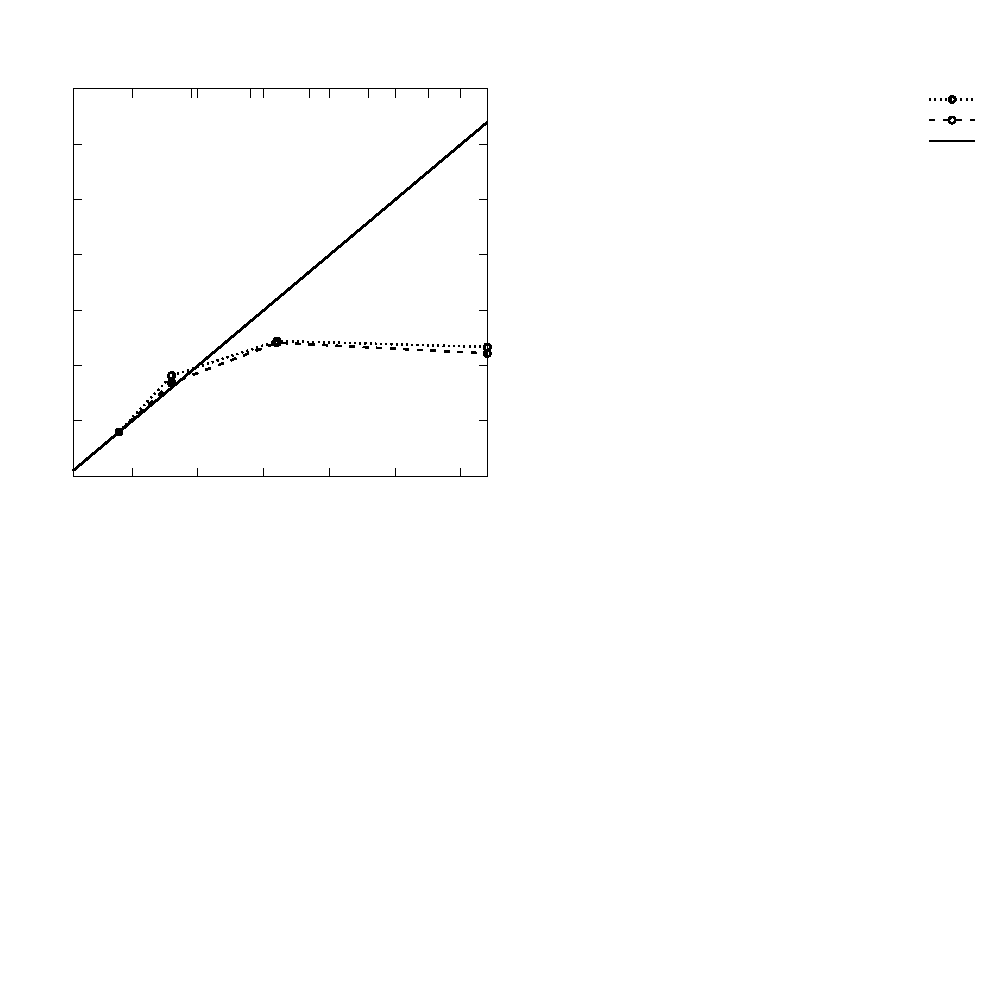
\includegraphics{Additional_2}}%
    \gplfronttext
  \end{picture}%
\endgroup
